% Two Column Article documento class
\documentclass[12pt]{article} 

% package includes
\usepackage{sbc-template}
\usepackage[utf8]{inputenc} % encoding
\usepackage[brazil]{babel} % language
\usepackage{hyperref} % http links
\usepackage{natbib} % bibliograph
\usepackage{graphicx} % images
\usepackage{listingsutf8} % for code
\usepackage{color}
\usepackage[vlined,boxed,portuguese]{algorithm2e}
\usepackage{outlines}


% lstlisting definitions for coding
\lstset{
    tabsize=4,
    language=C,
    basicstyle=\ttfamily\footnotesize,
    aboveskip={1.5\baselineskip},
    columns=fixed,
    showstringspaces=false,
    extendedchars=true,
    breaklines=true,
    prebreak=\raisebox{0ex}[0ex][0ex]{\ensuremath{\hookleftarrow}},
    frame=single,
    numbers=left,
    showtabs=false,
    showspaces=false,
    showstringspaces=false,
    identifierstyle=\ttfamily,
    keywordstyle=\color[rgb]{0,0,1},
    commentstyle=\color[rgb]{0.000,0.392,0.000},
    stringstyle=\color[rgb]{0.627,0.126,0.941},
    numberstyle=\color[rgb]{0.545,0.270,0.074}
}


\sloppy


% Article title definitions 
\title{Análise e Gerenciamento de Rede através de Grafos em Redes Definidas por Software}


\author{Gustavo Pantuza, 
        Frederico Sampaio,
        Luiz F M Vieira, \\
        Dorgival Guedes,
        Marcos A M Vieira}
        

\address{Departamento de Ciência da Computação \\ 
         Universidade Federal de Minas Gerais
    \email{\{pantuza,fredmbs,lfvieira,dorgival,mmvieira\}@dcc.ufmg.br}
}


\date{25 de Novembro de 2013}


% Start of the document
\begin{document}

\maketitle
\begin{abstract}
\label{sec:asbtract}
Software Defined Networking (SDN) is an emergent architecture
that is dynamic, flexible, manageable and with low cost, 
consistent with the dynamics of the modern applications.
This architecture decouples the control plane from the data plane.
Tipically, networks are represented as graphs.
Based on it, this paper presents a network 
representation model using a graph through the control plane 
of a SDN controller.
Our SDN solution adopts OpenFlow protocol.
This project is based on POX, a SDN controller compatible 
with OpenFlow devices.
The graph aproach provides a global view of the network in real 
time and consistency.
The experiments show that the graph is a reliable representation of 
the real network and its events ocurred along time inside the network,
thus easing the management in Software Defined Networking.

\smallskip
\noindent {\bf Key Words:} Software Defined Networking, Graph, 
Network Management, OpenFlow, POX.
\end{abstract}
\begin{resumo}
\label{sec:resumo}
As redes definidas por software (SDN) representam 
uma arquitetura emergente dinâmica, 
flexível, gerenciável e de baixo custo,
condizente com a dinamicidade das aplicações atuais. 
Essa arquitetura desacopla o plano de controle do plano de dados. 
Redes tipicamente são representadas em forma de grafos.
Em função disso, esse trabalho apresenta
um modelo de representação da rede em grafos através do 
plano de controle de um controlador SDN. 
O protocolo \emph{OpenFlow} é um meio para construção de soluções em SDN.
Esse trabalho é baseado no POX, um controlador SDN compatível 
com dispositivos OpenFlow.
Essa abordagem em grafos fornece uma visão global da rede em tempo 
real e com consistência.
Os experimentos demonstram que o grafo proposto representa de 
maneira fiel o estado da rede assim como suas mudanças em função 
dos eventos ocorridos ao longo do tempo dentro da rede, 
facilitando assim, o gerenciamento em Redes Definidas por Software.

\smallskip
\noindent {\bf Palavras Chave:} Redes Definidas por Software, Grafos, 
Gerenciamento de redes, OpenFlow, POX.
\end{resumo}
\section{Introduction}
\label{sec:introduction}

%Software Defined Networks (SDN) decouple the data plane from control plane.
%\citep{guedes2012redes}.
Software environments designed to provide SDN applications
are named SDN controllers.
They have also been called network operating systems because they provide a layer
that
isolates and control the access to the physical network elements, providing
a standardized interface to them. That interface may take different forms,
like events in NOX~\cite{nox}, an internal database in Onix~\cite{teemu2010onix},
a predicate-rule based reasoning system~\cite{fml2009}, 
or a query language in Frenetic~\cite{Foster:2011:FNP:2034574.2034812},
for example.

No matter the API, 
almost all applications of Software Defined Networks (SDN)
need a topological view of the network; in
fact, that global view is one of the key aspects of that
paradigm~\citep{martin2010virtualizing}.
Graphs model the network topology in a direct, natural and precise way,
so describing the network using a graph has become a common practice in many works,
protocols and network software, including those on
SDN~\citep{ramya2012dynamic}.
In this sense, a graph should be a basic resource of an SDN controller,
providing the
network representation, the access and the control of the network elements in
a single structure. Thus, a graph module can be of multiple uses in this kind of
software.

%A controller is composed of many interconnected modules and can interact with external systems.
A graph model would be useful for both the internal modules of the
SDN controller as for the applications using the controller.
They need topological information or just access to the network data,
and the search for and access to the network
entities can be provided by the graph module. 
It may have the capacity to notify state changes, be it through events,
callbacks or other notification mechanisms.

Moreover, in practice, many SDN applications use graph algorithms to obtain
informations that affect the control of the underlying network, such as
Shortest Path, Minimum Spanning Tree, Graph Coloring, etc.
The graph module store this kind of representation directly and execute any
of those algorithms internally,
making the results available for other software modules,
with no need for them to repeat the
computation, and for the application developer to re-implement 
complex data structures and algorithms.
A graph module can be implemented for that goal, avoiding new dependencies
among different modules.


The interactions with the graph module can be encapsulated and 
defined as a semantically stable and standardized interface. Its implementation
can be modified to adjust to different systems, using different resources like
local memory, remote databases, centralized or distributed processing,
concurrency control, 
parallelism, persistence, performance and other relevant characteristics.

%Considering the importance of this field on network operating systems, including
%the management software and applications, 
%this paper aims to exemplify and analyze the utilization of graph modules on SDN development.
%The controller used in this work is POX. 
%
%As other SDN controllers, POX has no network representation built on graph.


This paper presents a
description of a new kind of abstraction for network management,
integrating elements like automated fault detection and provision for dynamic
graphs,
a real implementation on a system using OpenFlow~\citep{nick2008openflow},
and its experimental validation.

The remainder of this paper provides, first, a description of the POX controller
and the design, properties and project decisions that lead to the graph model
implementation.
After that we show some experiments and results obtained in a network simulation
environment, in this case, Mininet~\citep{lantz2010network}.
Finally, we discuss some paths for future work and a brief conclusion. 

\section{Trabalhos Relacionados}
\label{sec:related-work}

Um sistema de autenticação 
seguro é construído sobre o controlador SDN em \citep{james2013HyperPass}.
O projeto RouteFlow  \citep{christian2010openflow} 
descreve um modelo de apresentação topológica da rede 
através de arquivos de configuração.
Apesar de serem relacionados, 
principalmente por tratarem de questões de gerenciamento,
nenhum desses trabalhos foca a representação da rede em modelo de grafo.

\citep{martin2010virtualizing} apresenta um modelo
de controlador em que a rede lógica e a topologia real da rede podem 
ser mapeadas como grafos.
O projeto Onix da Google \citep{teemu2010onix} 
apresenta uma abordagem SDN em que o 
controlador mantém uma visão global da rede em forma de grafo.
A NIB - \emph{Network Information Base}, um dos elementos fundamentais 
do projeto Onix \citep{teemu2010onix},
é um banco de dados distribuído, 
garantindo consistência e escalabidade à aplicação.
Ambos se relacionam com o presente trabalho,
porém não focam o tema de grafos.

Em \citep{ramya2012dynamic}, é apresentado um módulo de 
grafos com capacidade de atualização dinâmica e uma API pública,
implementado em C++ usando STL (\emph{Standard Template Library}).
Ele possibilita a adoção de algoritmos gerais que podem ser executados 
sobre o grafo, entretanto foca algoritmos de computação de rotas e atribuição de caminho.
O trabalho é geral, porém sem integração com controladores SDN na prática.

No geral, a representação em grafos proposta no presente trabalho 
também mantém dados sobre a rede, similar à NIB do Onix.
Como é possível registrar dados ``extras'' para cada \emph{Entity}, 
o módulo \emph{graph} vai além de manter informações topológicas.
Inevitavelmente, a necessidade de se buscar e monitorar dados 
específicos, principalmente em redes complexas, atrai o design de software 
de SDN para a direção de alguma forma de linguagem (DSL) que simplifique, 
organize, generalize e garanta eficiência na manipulação desses dados.
Esse é o exemplo do Frenetic \citep{Foster:2011:FNP:2034574.2034812} 
e do Pyretic \citep{Monsanto:2013:CSN:2482626.2482629}.

Enquanto a abordagem da DSL é baseada em atuação, execução,
conjunta com o controlador,
o NIB é baseada em um banco de dados distribuído,
com uma abordagem mais ampla e atacando problemas mais gerais
como persistência, concorrência, redundância, escalabilidade, etc.

O POX, segundo seu mantenedor, Murphy Mccauley, 
adotou o modelo de \emph{network fabric} \citep{martin2012fabric}. 
Esta arquitetura propõe uma divisão lógica em que a rede possui três elementos: 
\emph{hosts}, \emph{edge switchs} e \emph{core fabric}. 
O POX foca sua atuação no \emph{core fabric}, que, 
segundo essa arquitetura, lida apenas com transporte básico de pacotes.
Por isso, a abordagem do presente trabalho também lida com
controladores SDN relacionados com o \emph{core fabric}, 
porém incluindo uma visão dos \emph{hosts} e, se necessário, dos \emph{edge switchs}.
Uma generalização para a Internet dessa arquitetura pode ser 
vista em \citep{barath2012software}. 

\section{O design do POX}
\label{sec:design}

Esta seção descreve as características mínimas e necessárias do POX 
para atingir o objetivo de elaboração do módulo de grafos.

O POX é um arcabouço para a elaboração de softwares de SDN.
Ele é baseado em componentes.
Os componentes arquiteturais do POX são chamados de módulos.
É possível carregar módulos tanto de forma estática (via {\it import})
quanto dinâmica, durante a execução (via {\it eval}). 
Cada módulo, representado por sua classe, 
se publica ao \emph{core} através de um método obrigatório chamado \emph{launch}.

O \emph{OpenFlow} \citep{nick2008openflow} é um protocolo de comunicação
que possibilita o acesso do plano de encaminhamento de um \emph{switch} 
ou roteador.
Esse acesso é feito através de uma interface padronizada para esses
dispositivos de rede.
Essa comunicação permite experimentar novos protocolos facilitando 
o desenvolvimento de pesquisas em redes.
O POX, um controlador SDN, implementa um componente para comunicar com 
dispositivos de rede que estão habilitados a utilizar o protocolo 
\emph{OpenFlow}. 
Esse componente chamado \emph{openflow}, é responsável por enviar 
comandos e receber mensagens dos equipamentos de rede. 
Para o núcleo do controlador essas mensagens e comandos ocorrem na 
forma de eventos.

O \emph{core} (núcleo) define o funcionamento do POX. 
Uma de suas principais funções é proporcionar a comunicação entre os módulos.
O principal mecanismo de comunicação é o envio de eventos.
O modelo de eventos torna o design mais flexível e com menor acoplamento.
O \emph{core} oferece um canal de eventos no modelo ``push'',
ou seja, ele recebe o evento dos \emph{publishers} e envia para os \emph{subscribers}.
Via \emph{core}, cada módulo pode publicar novos canais de eventos 
ou se inscrever em canais de eventos.
O próprio \emph{core} publica alguns canais de eventos, 
como os relacionados com a carga de módulos.

O POX contém alguns módulos de descoberta que 
publicam eventos que se relacionam com a topologia da rede.
Esses módulos foram criados em contextos diferentes. 
Um módulo específico, o \emph{topology},
é responsável por mapear a topologia da rede. 
Utilizando os recursos do \emph{core}, 
ele atua como uma espécie de canal de eventos canônico,
conectando vários \emph{publishers} diferentes com 
os diversos \emph{subscribers}, 
sem que um necessite conhecer o outro diretamente. 
Isso o torna um ponto central genérico
para os diferentes módulos de descoberta e controle da rede 
que podem ser adicionados ou removidos, 
dependendo do caso concreto,
sem afetar os módulos de gerenciamento e visualização da rede.

Um grafo que represente globalmente a rede 
deve contar com a integração do \emph{topology} com os
demais módulos relacionados. 
Ou seja, o grafo proposto pelo trabalho 
é uma representação da rede em tempo 
real e atualizado dinamicamente em função das informações notificadas 
pelo \emph{topology}. 

O \emph{topology} publica dois tipos de eventos:
entrada ({\it join}) e saída ({\it leave}) 
de entidades ({\it entity}).
A entidade é uma classe abstrata que pode ser
especializada em switch e host, por exemplo.
Os diversos módulos notificam os eventos ao \emph{topology},
via chamada direta de métodos \emph{addEntity} e \emph{removeEntity}. 
O topology, no papel de  {\it publisher}, notifica seus {\it subscribers}
por meio do mecanismo de eventos padrão do POX.

Contudo, tanto o \emph{topology} quanto diversos outros módulos relevantes
necessitaram de novos recursos, como novas classes, 
ajustes de eventos, informações e estruturas de dados adicionais, etc.
Por motivo de compatibilidade, durante os ajustes das classes já existentes no POX,
tentou-se afetar o mínimo possível os programas, principalmente as interfaces.
Os módulos relevantes para atingir os objetivos do presente trabalho são:

\begin{itemize}

\item{\emph{topology}}: 
Canal de eventos canônico que generaliza os eventos relacionados a topologia da SDN.
Ele determina uma chave única para cada entidade de rede no contexto do POX,
unificando a identificação entre diferentes módulos.
Modificado para incluir a entidade, e seus respectivos eventos, 
relacionados com \emph{links},
além do evento não implementados \emph{HostEvent}.

\item{\emph{host\_tracker}}: 
Seu objetivo é buscar e rastrear informações sobre os {\it hosts} dentro da rede.
Minimamente modificado, principalmente para tratar eventos de DHCP.

\item{\emph{openflow.topology}}: 
Um controle de topologia específico para switches OpenFlow.
Ele é integrado com o módulo \emph{topology} do POX.
Também foi modificado para incluir a notificação de eventos relacionados com \emph{links}.

\item{\emph{openflow.discovery}}: 
Identifica links entre switches OpenFlow por meio do protocolo LLDP.

\item{\emph{misc.dhcpd}}:
Servidor de DHCP para configuração dinâmica da rede IP.

\end{itemize}

Outras questões relacionadas como, desempenho, estabilidade,
distribuição, balanceamento de carga, redundância, 
escalabilidade também vão além tanto do objetivo quanto da
implementação do POX ou de seus módulos.
É fundamental destacar que o POX, 
assim como diversos outros softwares de SDN, 
tem objetivos relacionados com a pesquisa científica, 
incluindo exemplos de conceitos e aplicações.
Seu objetivo e o estágio atual não é de software 
capaz de atuar em ambiente complexos ou de produção,
principalmente no qual a estabilidade é um fator crítico.

\section{Decisões de Projeto}
\label{sec:project}
O sistema proposto está disponível em \, \url{https://github.com/pantuza/pox}.
Seguindo o design do POX, 
o módulo de grafos (\emph{graph}) se integra com 
os eventos relacionados à infraestrutura da rede,
que foram unificados no \emph{topology} e no \emph{host\_tracker}.
A integração do módulo \emph{graph} ocorre conforme a figura \ref{fig:design}.

\begin{figure}[h!]
    \centering
    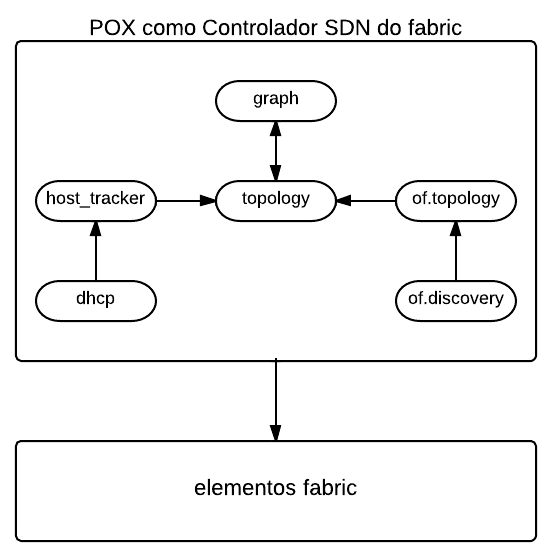
\includegraphics[scale=0.4]{fabric_design.png}
    \caption{integração entre os módulos}
    \label{fig:design}
\end{figure}

Seguem-se as principais decisões de projeto na implementação do sistema.

\subsection{Integração do \emph{host\_tracker} com o \emph{topology} e o \emph{misc.dhcpd}}

O \emph{host\_tracker} foi alterado para 
comunicar com o \emph{topology} através dos eventos de 
adicão ({\it join}) e remoção ({\it leave}) dos {\it hosts}. 
O \emph{host\_tracker}, ao descobrir mudanças no estado dos \emph{hosts} da rede, 
notifica o \emph{topology}. 
Por sua vez, o \emph{topology}, ao perceber mudanças na topologia da rede, 
informa o \emph{graph}, via evento, para que o grafo seja atualizado. 

Em suas contribuições recentes, o POX recebeu um módulo de DHCP. 
Esse módulo dispara eventos de \emph{DHCPLease} para o \emph{core} 
ao associar um IP para um \emph{host}.
Foi adicionado ao \emph{host\_tracker} um método para fazer escuta desse evento. 
Ao ser notificado, 
o método atualiza o dicionário python que mantém as informações dos hosts ativos. 
Essa alteração possibilita a descoberta antecipada de novos hosts na rede, 
otimizando a tarefa do \emph{host\_tracker}.

A integração entre \emph{host\_tracker} e \emph{topology} 
foi feita utilizando a estrutura de eventos que o POX possui. 
Assim, quando \emph{host\_tracker} recebe um evento de PacketIn, 
ele dispara um evento para o \emph{topology}, 
de maneira que o mesmo trate a entrada de um host na topologia da rede.
Esse evento (\emph{HostEvent}) foi implementado dentro do módulo \emph{topology} 
com o objetivo de manter a semântica por entidades (\emph{entity}). 
Assim, ao adicionar uma entidade ao \emph{topology}, se essa entidade é uma 
instância da classe \emph{Host}, então dispara-se o evento \emph{HostEvent}. 
O mesmo funcionamento é utilizado para a descoberta de \emph{switches} feita pelo
módulo \emph{openflow.topology} (módulo para descoberta de switches openflow)
que adiciona uma entidade da classe \emph{Switch} ao \emph{topology}.

Quando um vértice se torna inativo o módulo \emph{graph} é notificado
pelos módulos \emph{host\_tracker} e \emph{openflow.topology}.
Quando um \emph{switch} torna-se inativo, um evento de 
\emph{SwitchLeave} é disparado pelo \emph{openflow.topology} e o
módulo \emph{graph} pode atualizar o grafo representando a rede.
Essa identificação é feita através do protocolo LLDP e o evento 
é disparado imediatamente e o grafo atualizado.
Por sua vez, quando um \emph{host} está inativo, é necessário 
perguntar ao \emph{host} se ele ainda está ativo. 
Esse procedimento é feito pelo \emph{host\_tracker} que envia 
pacotes ARP para verificar a atividade do \emph{host}. 
Essa identificação é configurada no módulo \emph{host\_tracker}
que pode decidir a quantidade de pacotes ARP e a periodicidade 
dessa verificação. 
Assim, ao ser identificado que um \emph{host} está inativo 
o grafo é atualizado.

\subsection{Ajustes para incluir eventos relacionados com as arestas do grafo}

As arestas entre os \emph{hosts} e \emph{switches} são obtidas
indiretamente pelo evento de entrada e saída de \emph{host},
pressupondo um link necessário com o \emph{switch} diretamente conectado.
Nesse caso, é fundamental que o \emph{host\_tracker} informe 
o \emph{switch}, preferencialmente com o id 
ou o próprio objeto ``entidade'' do \emph{topology} e a porta da conexão.
Além disso, deve haver garantia que o \emph{host\_tracker} 
informe eventos de \emph{host} apenas quando estiver conectado
diretamente com o \emph{switch}.
Essas garantias já são consideradas na atual versão do \emph{host\_tracker}.

Outra forma de aresta do grafo ocorre entre os \emph{switches}.
Atualmente, o módulo \emph{openflow.discovery} controla os 
links entre \emph{switches} OpenFlow. 
Ele publica o evento \emph{LinkEvent} que notifica 
a entrada ({\it up} ou descoberta) e saída ({\it down} ou deleção)
dos links.
O módulo \emph{openflow.topology} atua como {\it subscriber} desse evento
e faz as atualizações necessárias nos dados do \emph{switch}.
Contudo, essa mudança de estado não é notificada para o \emph{topology}.
Esse é um ponto que foi necessário modificar a interface e os
eventos do \emph{topology}.
Para isso, foi adicionada a ``entidade'' \emph{Link} (subclasse) e
os eventos \emph{LinkJoin} e \emph{LinkLeave}.
O objeto \emph{Link} é composto de duas portas,
uma de cada \emph{Entity} conectada,
no caso, apenas \emph{switches}.


\subsection{Modelagem do grafo}
O grafo proposto pelo presente trabalho é representado por
$G=(V,A)$, no qual $V$ e $A$ são os conjuntos de vértices e arestas, respectivamente. 
 $V$ e $A$, são finitos.
Cada vértice $v \in V$ pode representar um \emph{host} ou um
\emph{switch} na rede. 
Cada aresta $u \to v \in A$ representa um link entre dois vértices.
As arestas possuem um peso $g(u, v)$ que descreve o volume de 
tráfego em bytes recebidos e transmitidos através da aresta/\emph{link}. 

Cada vértice é um objeto das classes \emph{Host} ou \emph{Switch},
logo, por herança são objetos da classe \emph{Entity}. 
Em função disso é possível identificar dentro do módulo 
\emph{graph} qual o tipo do vértice corrente. 
O peso das arestas é obtido através da leitura dos contadores 
de fluxos presentes nos \emph{switches openflow}.
Para o módulo \emph{graph} são lidos os contadores de fluxo da porta 
no switch. 
A lista de contadores é apresentada na Tabela \ref{tbl:counters} e em 
\citep{openflow2013protocol}.
Através da contagem desses fluxos é possível mensurar o tráfego 
decorrente na aresta/\emph{link}.

\begin{table}[h!]
    \centering
    \begin{tabular}{| l | l |}
    \hline
    \textbf{Contador} & \textbf{Bits} \\ \hline
    Pacotes Recebidos & 64 \\ \hline
    Pacotes Transmitidos & 64 \\ \hline
    Bytes Recebidos & 64 \\ \hline
    Bytes Transmitidos & 64 \\ \hline
    Drops Recebidos & 64 \\ \hline
    Drops Transmitidos & 64 \\ \hline
    Erros Recebidos & 64 \\ \hline
    Erros Transmitidos & 64 \\ \hline
    Erros de Frames Recebidos & 64 \\ \hline
    Erros de Transbordo Transmitidos & 64 \\ \hline
    Erros de CRC Recebidos & 64 \\ \hline
    Colisões & 64 \\
    \hline
    \end{tabular}
    \caption{Contadores de fluxos por Porta}
    \label{tbl:counters}
\end{table}

\subsection{Elaboração do módulo \emph{graph}}

As modificações descritas completam os requisitos necessário para o módulo \emph{graph},
em especial o controle de eventos que afetam os vértices e arestas do grafo.
Através das informações topológicas fornecidas pelos eventos do \emph{topology},
a classe \emph{graph} mantém, em memória, um grafo atualizado em tempo real. 
A instância dessa classe é \emph{subscriber} dos eventos do módulo \emph{topology}. 
Dessa forma, recebe-se eventos de qualquer um dos {\it publishers} 
do canal de eventos canônico do \emph{topology}, 
incluindo o \emph{openflow\_discovery} e \emph{host\_tracker}. 

\subsection{Interface de programação (API)}

O \emph{graph} possui uma interface (API) para que outros módulos do 
controlodor possam requisitar informações da topologia da rede. 
É possível imaginar aplicações como balanceamento de carga ou roteamento
que utilizem informações contidas no grafo.

\begin{outline}
\0 Os Métodos com dados do grafo são:
    \1 \emph{get\_vertex(id)}:
    Retorna uma entidade do grafo identificada (id dado pelo \emph{topology}).
    \1 \emph{get\_adjacents(id)}: 
    Retorna os nós (vértices) imediatamente adjacentes ao nó com identificado.
    \1 \emph{snapshot()}: 
    Retorna uma cópia do grafo, em forma de duas coleções, 
    uma de vértices (nós) e outra de arestas.
    \1 \emph{to\_dot(harq, layout = "dot")}: 
    Grava uma cópia do grafo para ser processada pelo Graphviz
    \citep{john2003graphviz}.
\0 Os Algoritmos de grafos já implementados são:
    \1 \emph{get\_mst()}:
    Retorna uma árvore geradora mínima do grafo (\emph{minimum spanning tree})
    em tempo real. A árvore é computada sempre que o grafo é atualizado.
\end{outline}


\subsection{Simulação via Mininet}

O funcionamento do módulo \emph{graph} do POX foi testado no Mininet,
\citep{lantz2010network}
um software de simulação de rede amplamente usado, 
principalmente para controladores SDN.
O Mininet, assim como o POX, é implementado em Python.
Também foi necessário acrescentar recursos para viabilizar o uso do Mininet,
especialmente métodos de adição e remoção de elementos na rede,
uma vez que os grafos devem ser mantidos de forma dinâmica.
Apesar de ser amplamente programável, 
as remoções e inserções dinâmicas de entidades de rede 
não eram disponibilizadas no Mininet,
principalmente depois de estabelecida a topologia inicial 
e da rede entrar em funcionamento.
Boa parte do esforço  análise detalhada dos algoritmos e das estruturas de dados usadas 
no controle do Mininet, foram implementados e testados diversos métodos.
A compatibilidade também foi o principal fator das alterações feitas,
mantendo-se sempre as estruturas e interfaces originais do Mininet.
Além das interfaces de código, que tiveram reflexo em várias classes, 
a interface de comandos padrão (\emph{prompt}) do Mininet
foi estendida para os novos comandos de adição e remoção dinâmica de controladores,
 \emph{switches}, \emph{hosts}, \emph{links} e interfaces de rede.
\section{Experimentos}
\label{sec:experiments}

O objetivo dos experimentos é validar e avaliar o sistema proposto.
Considere-se uma rede com uma topologia simples conforme mostrado abaixo: 

\begin{figure}[h!]
    \centering
    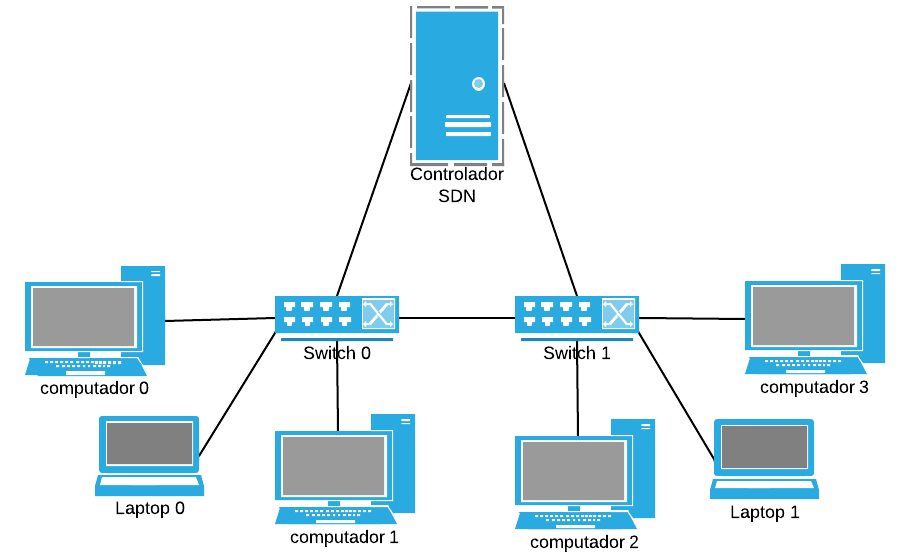
\includegraphics[scale=0.4]{mininet_topology.png}
    \caption{Topologia simples}
    \label{fig:topology}
\end{figure}

Conforme pode ser visto na figura \ref{fig:topology}, tem-se seis \emph{hosts} em sub-redes diferentes. 
Os dois \emph{switches} são controlados pela mesma instância do controlador 
POX.
Essa topologia foi configurada através do \emph{mininet} \citep{lantz2010network}. 
O mininet permite a criação de \emph{scripts} que geram topologias 
na rede simulada. 
Note que, na topologia proposta, existe um \emph{link} entre os dois 
switches.
Esse \emph{link} também é representado por uma aresta no modelo do grafo
proposto.


\subsection{Detecção de entidades}
O sistema inicia o grafo da rede vazio.
Os \emph{switches} são os primeiros a serem identificados. 
Como o controlador está ligado diretamente a eles pela interface 
\emph{OpenFlow}, um evento de \emph{ConnectionUp} é disparado 
pelo núcleo do controlador.

\begin{figure}[h!]
\centering
\begin{lstlisting}
INFO:topology.graph:SwitchJoin id: 2
INFO:topology.graph:SwitchJoin id: 1
INFO:topology.graph:1, 2
DEBUG:openflow.discovery:Dropping LLDP packet 275
INFO:topology.graph:LinkEvent fired
INFO:host_tracker:Learned 1 1 7e:e6:9b:89:39:2e got IP 10.0.0.1
INFO:topology.graph:HostJoin id: 7e:e6:9b:89:39:2e
INFO:host_tracker:Learned 2 1 62:77:44:24:13:49 got IP 10.0.0.2
INFO:topology.graph:HostJoin id: 62:77:44:24:13:49
\end{lstlisting}
\caption{Detecção de entidades}
\label{fig:detection}
\end{figure}

Nas duas primeiras linhas do \emph{log} mostrado na figura
\ref{fig:detection}, o módulo \emph{graph} foi notificado
da descoberta de dois \emph{switches} na rede.
A \emph{callback} do evento \emph{SwitchJoin} adiciona um vértice ao grafo. 
Assim, dois vértices do tipo \emph{switch} foram referenciados no grafo. 
Na linha 5, nota-se que a descoberta de um \emph{link} (entre switches).
O módulo \emph{openflow.discovery}, através do protocolo LLDP identificou 
o link entre \emph{switches}.
O grafo foi notificado e estabeleceu uma aresta entre os 
vértices (\emph{switches}).
As linhas 7 e 9 mostram a descoberta de dois hosts. 
Esses hosts foram descobertos pelo módulo \emph{host\_tracker} via 
escuta dos eventos de DHCP.
É importante ressaltar que a descoberta de \emph{hosts} também ocorre 
independente do DHCP.
Um novo pacote que passa por um \emph{switch} e não possui regra
instalada na tabela de fluxos é encaminhado ao controlador que 
dispara um evento de \emph{PacketIn}. 
Para tal, o \emph{host\_tracker} se encarrega de escutar esse evento 
e notificar o grafo através do evento \emph{HostJoin}.
O grafo, ao ser notificado, cria vértices para esses \emph{hosts} associando uma
aresta entre eles e o \emph{switch} ao qual eles estão conectados.
Dessa forma as entidades da rede são identificadas e computadas no grafo.

\subsection{Remoção de entidades}
Foram executados dois experimentos para validar a atualização do grafo
quando uma entidade (\emph{host/switch}) torna-se inativo/inalcançável.
Para o caso de remoção de \emph{host}, foi desligada a interface de 
rede de um \emph{host} via \emph{prompt} de comandos do mininet. 
O \emph{host\_tracker}, após um tempo fixo (\emph{timerInterval}) 
verifica via ARP Ping se os \emph{hosts} estão ativos.
Para esse cenário da remoção de um \emph{host}, após 30 segundos o 
\emph{host\_tracker} identificou a inatividade do \emph{host} e 
disparou o evento de \emph{HostLeave}, atualizando assim o grafo.
Para o caso do \emph{switch}, através do mininet, foi desligado um 
dos switches da topologia da figura \ref{fig:topology}.
O controlador está ligado diretamente ao \emph{switch}. 
Assim, ao ser desligado, o \emph{core} do POX dispara um evento 
de \emph{SwitchLeave} ao qual o módulo \emph{graph} está inscrito. 
Logo, o grafo é atualizado removendo o vértice do \emph{switch} e dos
\emph{hosts} ligados a ele. 

\subsection{Visualização em tempo real da rede}
Na figura \ref{fig:full_graph} é apresentado parte do grafo de uma rede
com 8 \emph{switches}, cada um com 30 \emph{hosts} conectados totalizando
248 entidades na rede.
Esse grafo é atualizado em tempo real em função dos eventos de rede ocorridos 
dentro do controlador, como entrada e saída de entidades, volume de tráfego 
na rede entre outros citados nesta seção. 

\begin{figure}[h!]
    \centering
    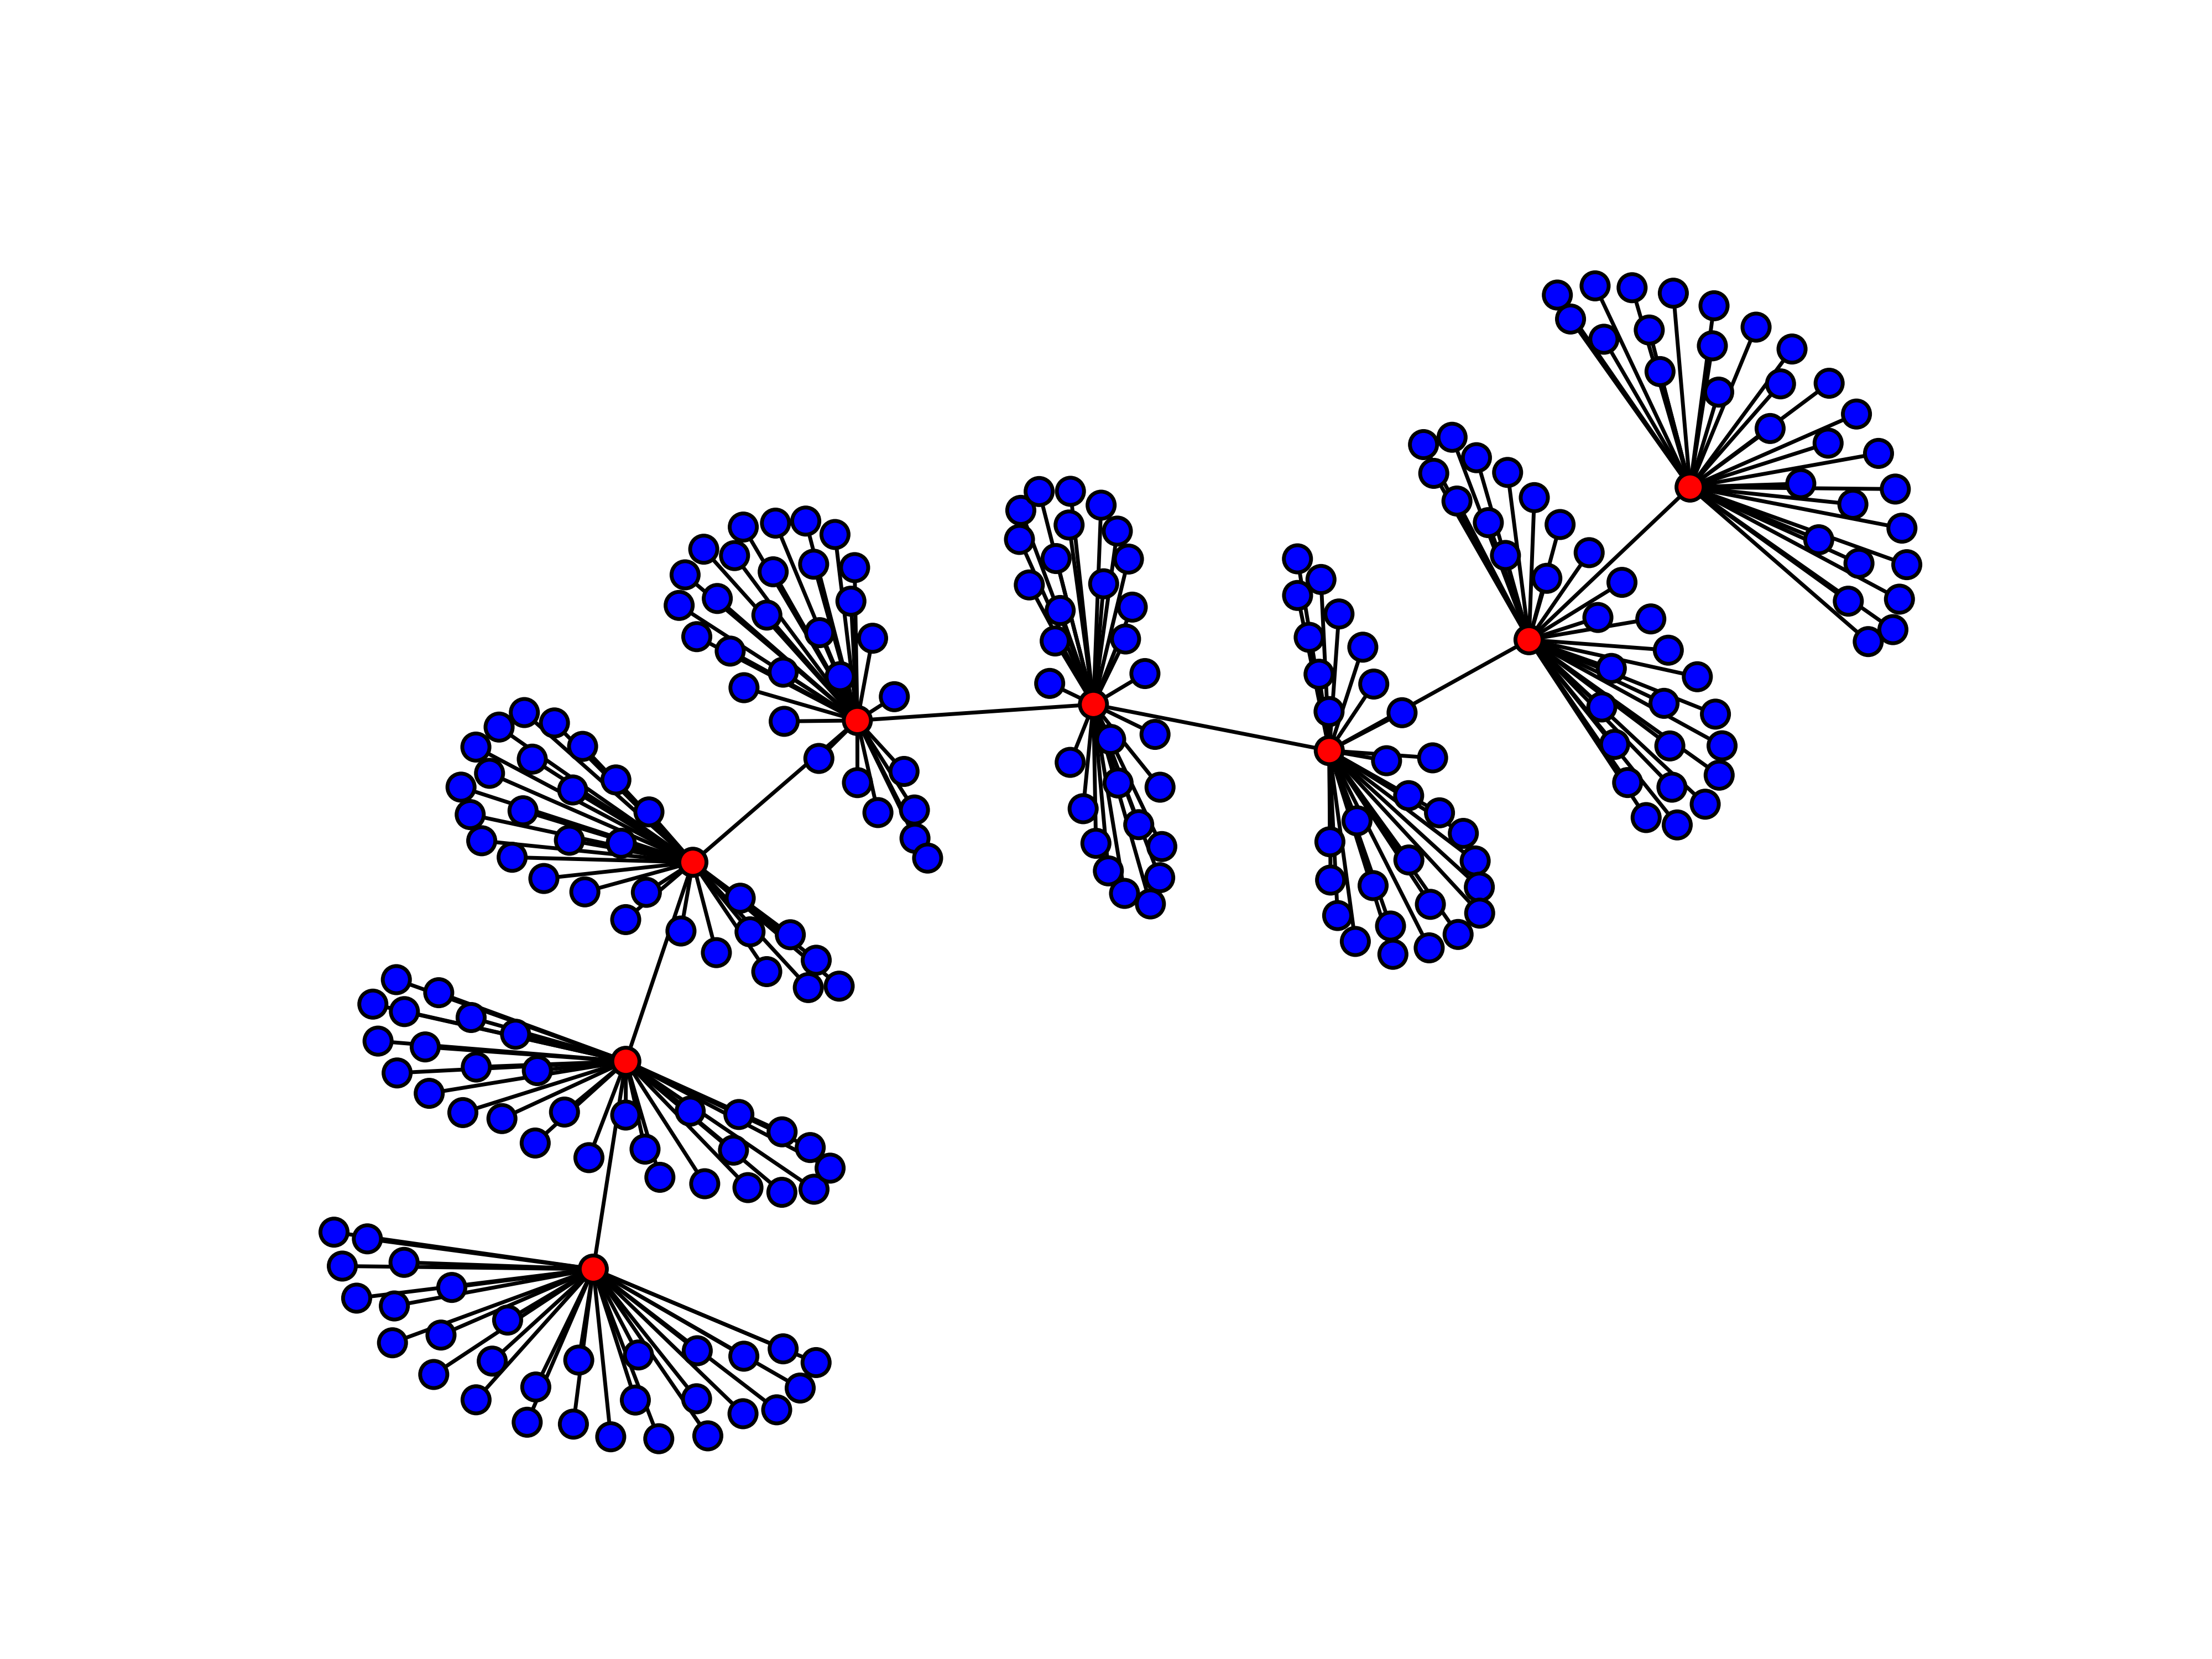
\includegraphics[scale=0.5]{full_graph.png}
    \caption{Grafo representando uma grande rede}
    \label{fig:full_graph}
\end{figure}

\subsection{Identificação de tráfego na rede}
Para computar o tráfego (TCP) na rede foi executado o programa \emph{iperf} 
como servidor no \emph{host} 'Host 0a' utilizando a topologia apresentada
na figura \ref{fig:topology}.
O \emph{host} 'Host 1e' conecta-se como cliente. 
Conformo pode ser notado na figura \ref{fig:iperf}, o tráfego 
em bytes na arestas desses \emph{hosts} é superior ao demais \emph{hosts}.
No momento em que foram lidos os contadores \emph{OpenFlow} e computados
os pesos das arestas, obteve-se um tráfego de 55894 bytes através do caminho
entre os dois \emph{hosts} citados.
Os valores apresentados para os demais \emph{hosts} (41 bytes) são referentes
ao tráfego ARP PING disseminado pelo módulo \emph{host\_tracker}
O experimento com o \emph{iperf} mostrou uma taxa de envio 
(\emph{throughput}) entre os \emph{hosts} de 300 Mega bits por segundo.

\begin{figure}[h!]
    \centering
    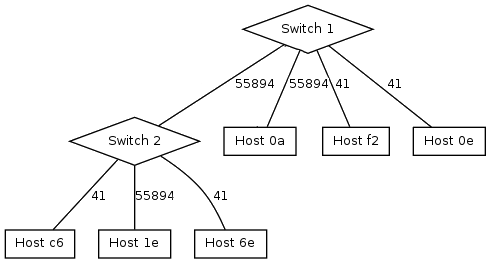
\includegraphics[scale=0.8]{graph_iperf.png}
    \caption{Tráfego TCP (em bytes) entre os hosts ’Host 1e’ e ’Host 0a’}
    \label{fig:iperf}
\end{figure}

\subsection{Árvore Geradora Mínima}
Uma árvore geradora mínima é mantida em tempo real sobre o grafo
da rede. 
Quando o grafo adiciona, remove ou atualiza arestas/vértices a árvore 
geradora mínima é computada. 
Outros módulos podem utilizá-la através da API do módulo em grafos.

Árvores geradoras mínimas são essenciais em diversas tarefas no gerenciamento
de redes.
Tarefas como disparar 'alarmes' quando a árvore estiver desconexa ou 
contenha \emph{loops}, conforme mostrado em \citep{schmid2013exploiting}.
É possível imaginar um sistema distribuído que consulte a árvore geradora
mínima para executar um algoritmo de propagação de mensagem \emph{flood} 
de maneira inteligente e menos custosa para 
a rede \citep{Monsanto:2013:CSN:2482626.2482629}.
Uma rede com múltiplos \emph{switches} pode implementar um 
balanceamento de carga eficiente que considere o tráfego nas arestas
utilizando a árvore geradora mínima em tempo real.
Além disso, é possível imaginar soluções como o \emph{Green MST}, 
apresentado em \citep{prete2012energy}. 
Uma abordagem em SDN utilizando uma árvore geradora mínima 
para reduzir o consumo elétrico da rede utilizando métricas da 
camada de aplicação. 

% \section{Discussões relevantes}
\label{sec:discussions}

Atuamente, protocolos de controle de tráfego em rede interna (\emph{core fabric}),
como o OSPF e o IS-IS, já mantêm uma representação de grafo da rede.
Os controladores SDN podem usar estes protocolos para abstrair o 
fluxo da rede interna.
Contudo, esses protocolos também podem ser implementados diretamente
no controlador SDN.
Além disso, pode-se considerar cenários de controle totalmente diferentes
como, por exemplo, controles baseados em MPLS, 
incluindo o conceito de rótulos e circuitos virtuais.
Essa é uma das principais vantagens da SDN, fornecer meios de implementação,
testes e avaliação de novos planos de controle, principalmente para 
uma rede interna, ou com alguma forma de administração interna específica.
Nesse contexto mais geral, recursos de representação em grafos podem ser 
mais do que relevante, podem ser uma necessidade.



\section{Future work}
\label{sec:future}

As a future work we plan to build an on-line graph visualizer 
that interacts with the network administrator and shows, in 
an easier way, the entire network operation.
Just like POX, if the controller process is terminated, then the
entire graph is lost.
For that, a distributed graph database can be used to store
the network graph in a persistent, reliable and fault tolerant
structure.
Default graph algorithms should be given by the graph module. 
These algorithms could be configured to run in predefined 
period.
\section{Conclusão}
\label{sec:conclusion}

O presente trabalho apresentou o uso de grafos
no contexto de uma SDN, por meio do POX e
em ambiente de simulação fornecido pelo \emph{mininet}.
Foram descritos também, vários aspectos relacionados a arquitetura e design 
tanto do POX quanto do \emph{mininet}.
Manter um grafo da rede em tempo real com atualizações dinâmicas vai
diretamente de encontro com uma das principais vantagens em se 
desacoplar o plano de controle do plano de dados que é obter uma 
visão global da rede,  
além de compor um ótimo sistema para que outras aplicações 
possam utilizá-lo.
Foi mostrado, nos experimentos, que o sistema mantém um estado fiel, 
consistente e dinâmico da rede real, 
facilitando a tarefa de gerenciamento de um rede definida por 
software.

% Import bibliograph file
\bibliographystyle{sbc}
\bibliography{references}

\end{document}